
All'interno dell'intensa campagna di studi condotta per verificare se le soluzioni previste per il progetto NUMEN possano garantire le prestazioni richieste, è stato svolto ad Aprile 2019 un test beam sui primi due prototipi di telescopi basati sulla tecnologia SiC-CsI.
Tale test si è tenuto ai Laboratori Nazionali del Sud (LNS) utilizzando un fascio di particelle di \ce{^{20}Ne} a 20~AMeV, prodotto dal Ciclotrone Superconduttore K800.
Al fine di favorire la generazione degli ioni di interesse per NUMEN, ovvero Ossigeno, Fluoro e Neon, si è scelto di utilizzare un bersaglio di \ce{^{12}C} da 400~$\mu$g/cm\ap{2}.

Il test aveva lo scopo di valutare la risposta dei telescopi e di confrontare l'elettronica tradizionale di MAGNEX con la nuova elettronica VMM3a~\cite{degeronimo:ieee13} per il progetto.
In questo capitolo vengono presentati i risultati ottenuti durante tale test e viene mostrato il confronto tra questi e i dati prodotti attraverso le simulazioni implementate per questo lavoro di tesi. 
Dal momento che i prototipi utilizzati nel test presentano alcune differenze rispetto ai telescopi che verranno impiegati per NUMEN, è stato necessario modificare alcuni parametri della simulazione: in primo luogo, ricordando che, in uno dei due dispositivi (Tel~A), il primo stadio era montato in configurazione reverse, il substrato epitassiale del rivelatore al SiC è stato posto davanti al volume sensibile.
Inoltre, le dimensioni trasversali e gli spessori delle diverse componenti sono state cambiate in modo da riprodurre le caratteristiche descritte nel Paragrafo~\ref{par:telescopi}.


\section{\iflanguage{italian}{I dati del telescopio SiC-CsI}{Data of SiC-CsI telescope}}


Gli eiettili prodotti nell'interazione fra proiettile e bersaglio, dopo aver attraversato il quadrupolo e il dipolo, giungono al rivelatore di piano focale (Focal Plane Detector, FPD) di MAGNEX, dove, in occasione del test, erano stati posti i due telescopi, chiamati Tel~A e Tel~B. 
Come descritto nella Sezione~\ref{sez:test}, insieme ai due telescopi, erano stati montati quattro dei rivelatori al silicio attualmente in uso, i quali servivano da riferimento e da confronto per la Particle IDentification (PID).

Poiché all'energia utilizzata nel test i prodotti di reazione non erano in grado di superare il substrato epitassiale del Tel~B, da tale telescopio era possibile estrarre soltanto il segnale sulla perdita di energia, non permettendo di riprodurre le correlazioni $\Delta E - E_{resid}$ utili per l'identificazione in numero atomico $Z$ degli ioni.
Di conseguenza, dal momento che questo lavoro aveva lo scopo di studiare le performance di PID di tale sistema, sono stati analizzati soltanto i dati relativi al Tel~A.


%\subsection{\iflanguage{italian}{Le matrici $\Delta E_{SiC} - E_{CsI}$}{$\Delta E_{SiC} - E_{CsI}$ matrices}}

In Figura~\ref{fig:sic_csi_standard} è riportata la matrice $\Delta E_{SiC} - E_{CsI}$ registrata dal Tel~A utilizzando l'elettronica standard (si veda il Paragrafo~\ref{par:elettr_standard}): come si può notare i luoghi dei diversi ioni appaiono ben separati in una regione che va dal Boro (B) al Neon (Ne).
Si può, inoltre, osservare che, poiché ai fini della PID non è necessario utilizzare la correlazione $\Delta E_{SiC} - E_{tot}$, i rivelatori non sono stati calibrati e, conseguentemente, le variabili $\Delta E_{SiC}$ e $E_{CsI}$ sono misurate in canali.


\begin{figure} [!p]
	\centering
	\includegraphics[width=\textwidth, keepaspectratio]{Grafici_Tesi2/Confronto/desic_ecsi.png}
	\caption{Le correlazioni $\Delta E_{SiC} - E_{CsI}$ ottenute dal Tel~A durante il test utilizzando la catena elettronica standard. La linea nera indica il taglio grafico effettuato per la selezione in numero atomico dell'Ossigeno.} \label{fig:sic_csi_standard}
\end{figure}




%Alla luce di questo risultato, il telescopio SiC-CsI sembra, dunque, rispondere alle richieste del progetto.
%Ricordando che questo telescopio era montato in configurazione reverse, si può anche osservare che il substrato epitassiale da 100~$\mu$m non sembra influire negativamente sulle sue proprietà di identificazione. 

%Ciò consente, dunque, di selezionare 

%Per confrontare le prestazioni di questo sistema con quelle solitamente ottenute utilizzando la co


%A questo punto può essere utile confrontare le prestazioni di questo sistema con quelle dell'apparato standard di MAGNEX, nel quale l'identificazione in numero atomico degli ioni avviene correlando la misura dell'energia persa $\Delta E$ nel gas con quella dell'energia residua $E_{resid}$ nei rivelatori al silicio; in particolare, la perdita di energia nel gas è data dalla somma delle sei perdite di energia $\Delta E_i$ misurate dai fili proporzionali.
%Inoltre, dal momento che la perdita di energia dipende dalla lunghezza della traiettoria dello ione all'interno del FPD, essa viene corretta, evento per evento, moltiplicando per il coseno dell'angolo di incidenza $\theta_{foc}$, ovvero 
%\begin{equation}
%	\Delta E^{corr}_{tot} \, = \, \frac{\cos \theta_{foc}}{\cos \theta_{tilt}} \, \sum_{i=1}^{6} \Delta E_i
%\end{equation}
%laddove $\theta_{tilt}$ rappresenta l'angolo di rotazione del FPD, pari a 59.2\textdegree.
In Figura~\ref{fig:sic_csi_vmm3a} si riporta la  matrice $\Delta E_{SiC} - E_{CsI}$ ottenuta con lo stesso telescopio utilizzando l'elettronica VMM3a (si veda il Paragrafo~\ref{par:elettr_vmm3a}): in questo caso si può notare che, sebbene si possano ancora riconoscere i luoghi corrispondenti ai diversi ioni, essi risultano parzialmente sovrapposti.
Ciò deriva da un maggiore contributo del rumore elettronico e da un peggiore accoppiamento fra i rivelatori e l'elettronica di front-end.
Ai fini della validazione delle simulazioni, si è scelto di analizzare soltanto quelli ottenuti utilizzando l'elettronica standard.

\begin{figure} [!p]
	\centering
	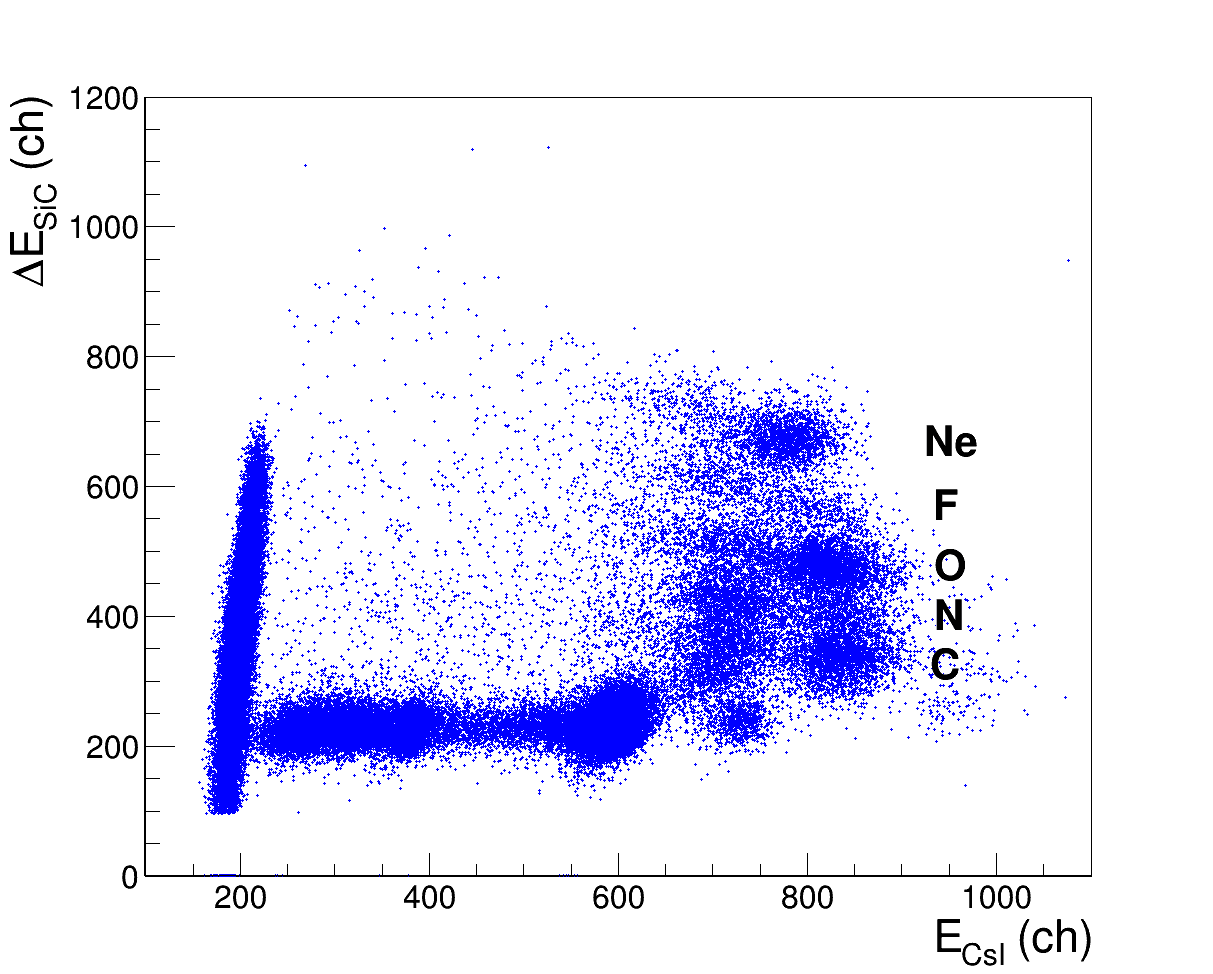
\includegraphics[width=\textwidth, keepaspectratio]{Grafici_Tesi/Test/matrice_sic_csi_vmm3a.png}
	\caption{Le correlazioni $\Delta E_{SiC} - E_{CsI}$ ottenute dal Tel~A durante il test utilizzando l'elettronica basata sul chip VMM3a.} \label{fig:sic_csi_vmm3a}
\end{figure}

\section{\iflanguage{italian}{Analisi dei dati del test beam}{Analysis of test beam data}}

Per poter confrontare i dati sperimentali con i risultati delle simulazioni è necessario che queste riproducano nel modo più fedele possibile le condizioni sperimentali.
Dunque, è stata svolta un'analisi dei dati raccolti durante il test per estrarre delle informazioni da inserire opportunamente nella simulazione.
In primo luogo, è necessario stabilire quali ioni debbano costituire le particelle primarie simulate, per cui è stata svolta un'identificazione dei prodotti di reazione.
%Inoltre, poiché l'energia delle particelle primarie è un parametro di fondamentale importanza, è stata determinare l'energia con cui gli ioni incidevano sul telescopio.
%%Inoltre, dal momento che un altro parametro di fondamentale importanza riguarda l'energia di tali particelle, è stata condotta un'analisi per determinare l'energia di incidenza degli ioni sul telescopio.


%Ciò è stato possibile grazie alla correlazione tra posizione ed energia indotta dalla forza di Lorentz: 

\subsection{\iflanguage{italian}{Identificazione dell'\ce{^{16}O}}{Identification of \ce{^{16}O}}}

A causa della bassa statistica raccolta durante il test, è stato deciso di simulare soltanto la specie atomica più abbondante nel campione.
%, che, come si può evincere dalla Figura~, risulta essere l'Ossigeno.
La prima fase nella procedura di identificazione consiste nel determinare il numero atomico $Z$ delle particelle rivelate: tale informazione è stata ricavata dalle matrici $\Delta E_{SiC} - E_{CsI}$ in Figura~\ref{fig:sic_csi_standard}, dove si può notare che la specie atomica maggiormente presente è l'Ossigeno (O). 

Dopo avere selezionato gli ioni O è necessario distinguerne gli isotopi in numero di massa $A$; a tale scopo, si è sfruttata la correlazione, indotta dalla forza di Lorentz, tra posizione ed energia: ricordando la~\ref{eq:legge_spettrometri_approx}, è possibile notare che la misura correlata di $x_{foc}$ ed $E$ permette di separare gli ioni in base al loro rapporto $\sqrt{m}/q$, laddove $m$ e $q$ rappresentano, rispettivamente, la massa e la carica della particella.
Nel caso del telescopio, la quantità~$E$ corrisponde con buona approssimazione a $E_{CsI}$.
La matrice $x_{foc} - E_{CsI}$ è mostrata in Figura~\ref{fig:xfoc2_csi_standard}, dove è possibile osservare che gli isotopi dell'O originati dall'interazione proiettile-bersaglio sono prevalentemente \ce{^{16}O}, \ce{^{17}O} e \ce{^{18}O}.
Si sottolinea che nella correlazione $x_{foc} - E_{CsI}$ il numero di massa cresce spostandosi verso sinistra poiché, per mantenere lo stesso valore di $x_{foc}$, se la massa aumenta $E_{CsI}$ deve diminuire.
Come si può notare dalla Figura~\ref{fig:xfoc2_csi_standard}, l'isotopo più abbondante dell'O presente nel campione è \ce{^{16}O}, la cui produzione è favorita poiché deriva da un processo di trasferimento di una particella $\alpha$ dal proiettile al bersaglio. 
La reazione scelta per la validazione della simulazione è, dunque, $^{12}\mbox{C}  ( ^{20}\mbox{Ne}, ^{16}\mbox{O} )  ^{16}\mbox{O} $.

\begin{figure} [!p]
	\centering
	\includegraphics[width=\textwidth, keepaspectratio]{Grafici_Tesi2/Confronto/xfoc_ecsi.png}
	\caption{Le correlazioni $x_{foc} - E_{CsI}$ ottenute, durante il test, dalla misura in correlazione del tracciatore e del rivelatore allo CsI . La linea nera indica il taglio grafico effettuato per la selezione in numero di massa dell'\ce{^{16}O}.} \label{fig:xfoc2_csi_standard}
\end{figure}



\subsection{\iflanguage{italian}{Determinazione dell'energia di eccitazione dell'\ce{^{16}O}}{\ce{^{16}O} excitation energy evaluation}}

%Una volta identificato l'isotopo, è necessario determinare l'intervallo di energia di eccitazione esplorato dal telescopio per il sistema eiettile-nucleo residuo; infatti, in base a quanto detto nel Paragrafo~\ref{par:particelle_primarie}, fissato lo ione, il dispositivo può vedere soltanto un certo range energetico, che dipende dalla sua estensione lungo la direzione dispersiva dello spettrometro.
%Il tool è stato, quindi, utilizzato per determinare tale range: sono stati simulati diversi livelli di eccitazione fino a quando 
%Per determinare tale range è stata la correla
%Tale range è stato determinato grazie all'utilizzo del tool: sono stati, infatti, simulati diversi livelli di eccitazione dell'\ce{^{16}O} e, tramite una scelta accurata, si è fatto in modo che due di questi passassero per gli estremi 


%Una volta identificato lo ione, è necessario verificare se tale ione giunge sul telescopio in uno stato eccitato.

Uno dei parametri da inserire nel tool di simulazioni è il range di energia di eccitazione del sistema eiettile-nucleo residuo.
Nel caso in esame, tale range è stato determinato attraverso il confronto tra i dati sperimentali e i risultati delle simulazioni, a diverse energie di eccitazione, prodotte dallo stesso tool.
Tale confronto è stato realizzato nella rappresentazione che correla l'angolo orizzontale $\theta_{foc}$ della traccia al piano focale e la coordinata orizzontale $x_{foc}$ del punto di arrivo dello ione sullo stesso piano.
In Figura~\ref{fig:tefoc_xfoc} è riportata la matrice $\theta_{foc} - x_{foc}$ relativa all'\ce{^{16}O}, laddove in rosso sono rappresentati i dati raccolti con il Tel~A, in blu quelli registrati con i rivelatori al silicio del FPD e in nero i dati simulati.


%Tale confronto è illustrato in Figura~\ref{fig:tefoc_xfoc}, dove si pu 

%Una volta identificato lo ione, si vuole individuare il range di energia di eccitazione del sistema eiettile-nucleo residuo esplorato dal telescopio; tale energia è, infatti, collegata all'energia cinetica dell'eiettile.





%Una volta identificato lo ione, è necessario verificare se il range di energia cinetica esplorato dal telescopio per tale ione corrisponde a processi in cui il sistema eiettile-nucleo residuo sia stato eccitato.
%A tal fine, è opportuno utilizzare la correlazione tra l'angolo orizzontale $\theta_{foc}$ della traccia al piano focale e la coordinata orizzontale $x_{foc}$ del punto di arrivo dello ione sullo stesso piano.
%In Figura~\ref{fig:tefoc_xfoc} è riportata la matrice $\theta_{foc} - x_{foc}$ relativa all'\ce{^{16}O}, laddove in rosso sono rappresentati i dati raccolti con il Tel~A, mentre in blu sono indicati quelli registrati con i rivelatori al silicio di MAGNEX.



\begin{figure} [!p]
	\centering
	\includegraphics[width=\textwidth, keepaspectratio]{Grafici_Tesi2/Confronto/tefoc_xfoc_energie.png}
	\caption{La matrice $\theta_{foc} - x_{foc}$ relativa all'\ce{^{16}O} ottenuta durante il test: in blu sono riportati i dati registrati con i rivelatori al silicio di MAGNEX, in rosso quelli raccolti con il Tel~A.} \label{fig:tefoc_xfoc}
\end{figure}








\section{\iflanguage{italian}{Confronto fra i dati del test e la simulazione}{Comparison between test data and the simulation}}

%La reazione scelta per il confronto è $^{12}\mbox{C}  ( ^{20}\mbox{Ne}, ^{16}\mbox{O} )  ^{16}\mbox{O} $ a 400~MeV di energia di incidenza; inserendo i parametri rilevanti nel tool, tra cui gli ioni coinvolti, l'energia del fascio e il range di energia di eccitazione del sistema eiettile-nucleo residuo, 
%Noti tutti i parametri da inserire nel tool, è stata svolta una simulazione 



I dati simulati sono stati elaborati dalla macro di post-processing, allo scopo di ricostruire gli spettri da comparare con i dati sperimentali.
È bene precisare che prima di effettuare il confronto è necessario uniformare le unità di misura; infatti, mentre le distribuzioni energetiche ricavate dalla simulazione sono già espresse nell'opportuna grandezza, gli spettri sperimentali devono essere calibrati.
A tal fine, sono stati utilizzati i dati relativi allo scattering elastico del \ce{^{20}Ne} su bersaglio di \ce{^{197}Au}, per il quale i campi magnetici del dipolo e del quadrupolo sono stati opportunamente fissati facendo in modo che una parte degli ioni scatterati arrivasse sul telescopio.
È stata, dunque, svolta un'analisi per determinare l'energia cinetica incidente, nota la quale è stato possibile stimare il deposito energetico del \ce{^{20}Ne} nel rivelatore al~SiC e nel cristallo di~CsI.
Tale stima è stata effettuata utilizzando LISE++~\cite{tarasov:nimb08}, software nato per simulare la produzione di fasci di ioni attraverso meccanismi di reazioni nucleari.
La procedura di calibrazione ha permesso di calcolare la pendenza della retta di calibrazione senza fissarne l'offset; di conseguenza, quest'ultimo parametro è stato determinato sovrapponendo i centroidi delle distribuzioni sperimentale e simulata.

In Figura~ è riportato lo spettro simulato in $\Delta E_{SiC}$, messo a confronto con quello sperimentale: come si può notare, la compatibilità delle due distribuzioni è ragguardevole; in particolare, la simulazione riproduce correttamente la larghezza dello spettro sperimentale.
La risoluzione energetica dedotta dalla simulazione sembra, quindi, rispecchiare in modo fedele quella riscontrata nel test.
%Dal momento che tale quantità gioca un ruolo cruciale nella capacità di PID del telescopio
\begin{figure} [!p]
	\centering
	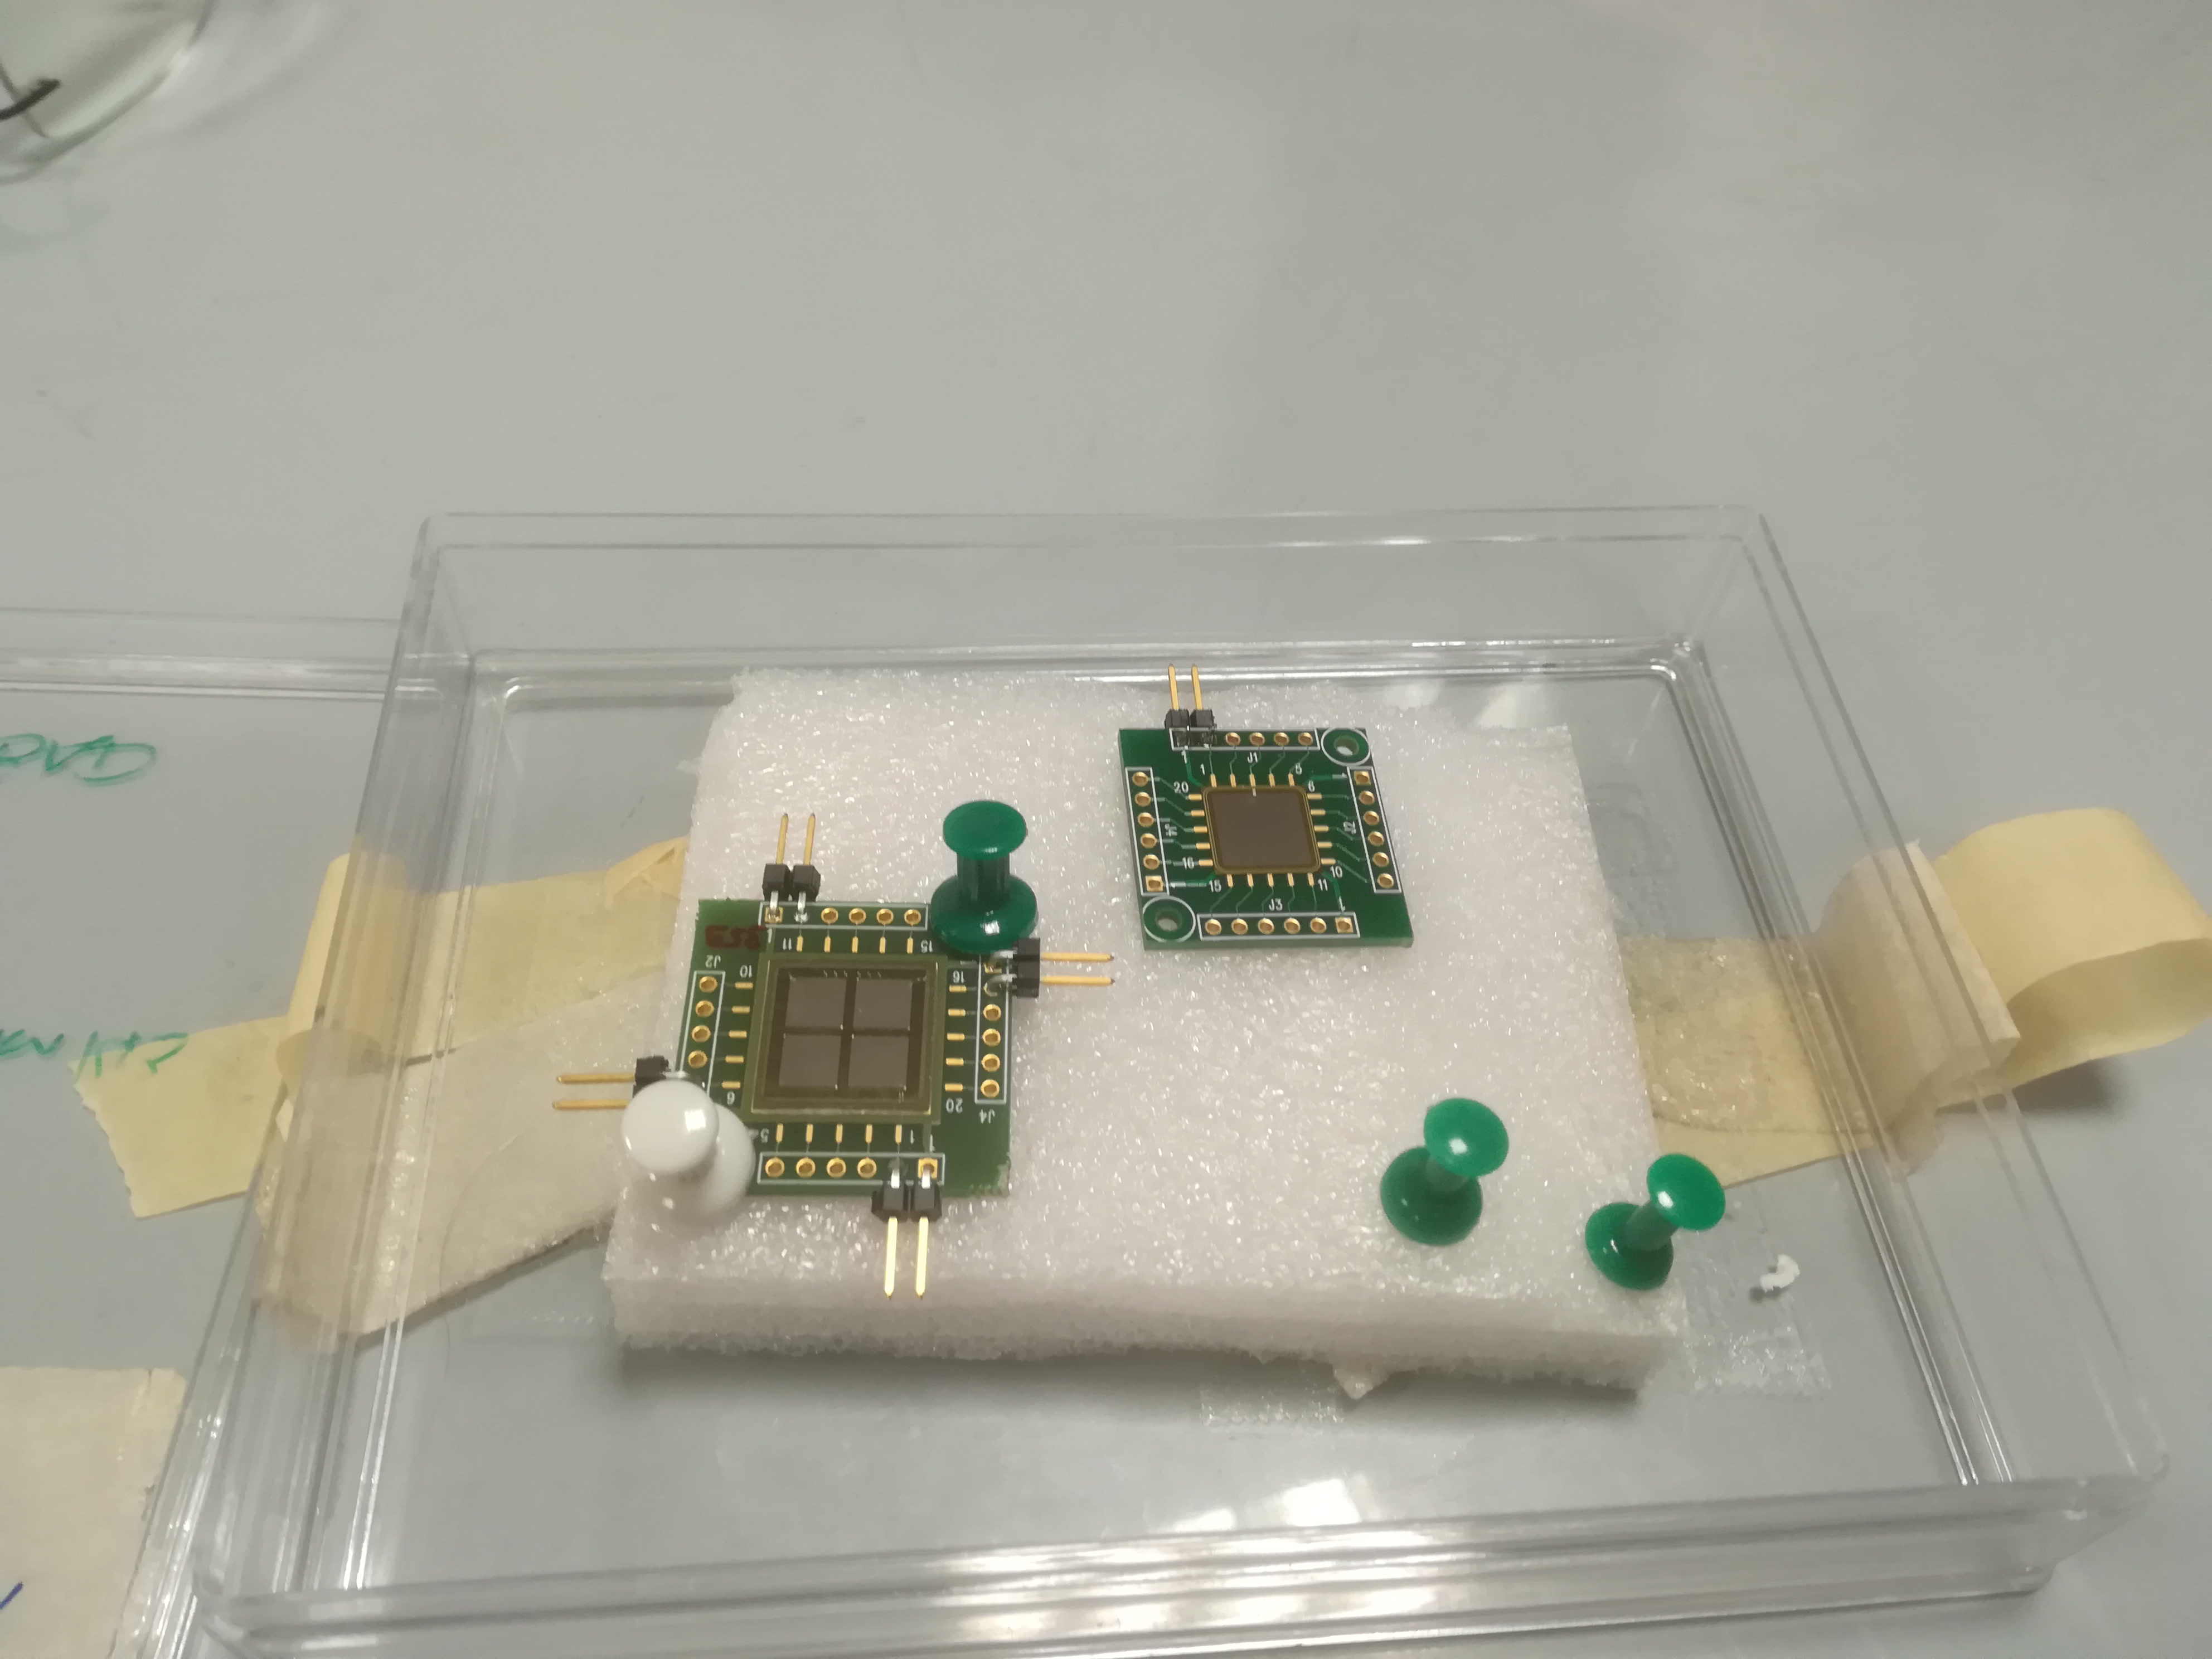
\includegraphics[width=\textwidth, keepaspectratio]{Grafici_Tesi2/Confronto/sic.png}
	\caption{Spettro in $\Delta E_{SiC}$: in blu sono rappresentati i dati sperimentali, in rosso quelli simulati. Gli istogrammi sono normalizzati in area.} \label{fig:spettro_sic_confronto}
\end{figure}

In Figura~ è illustrato il confronto tra lo spettro in $E_{CsI}$ simulato e quello sperimentale: anche in questo caso la compatibilità è significativa.


\begin{figure} [!p]
	\centering
	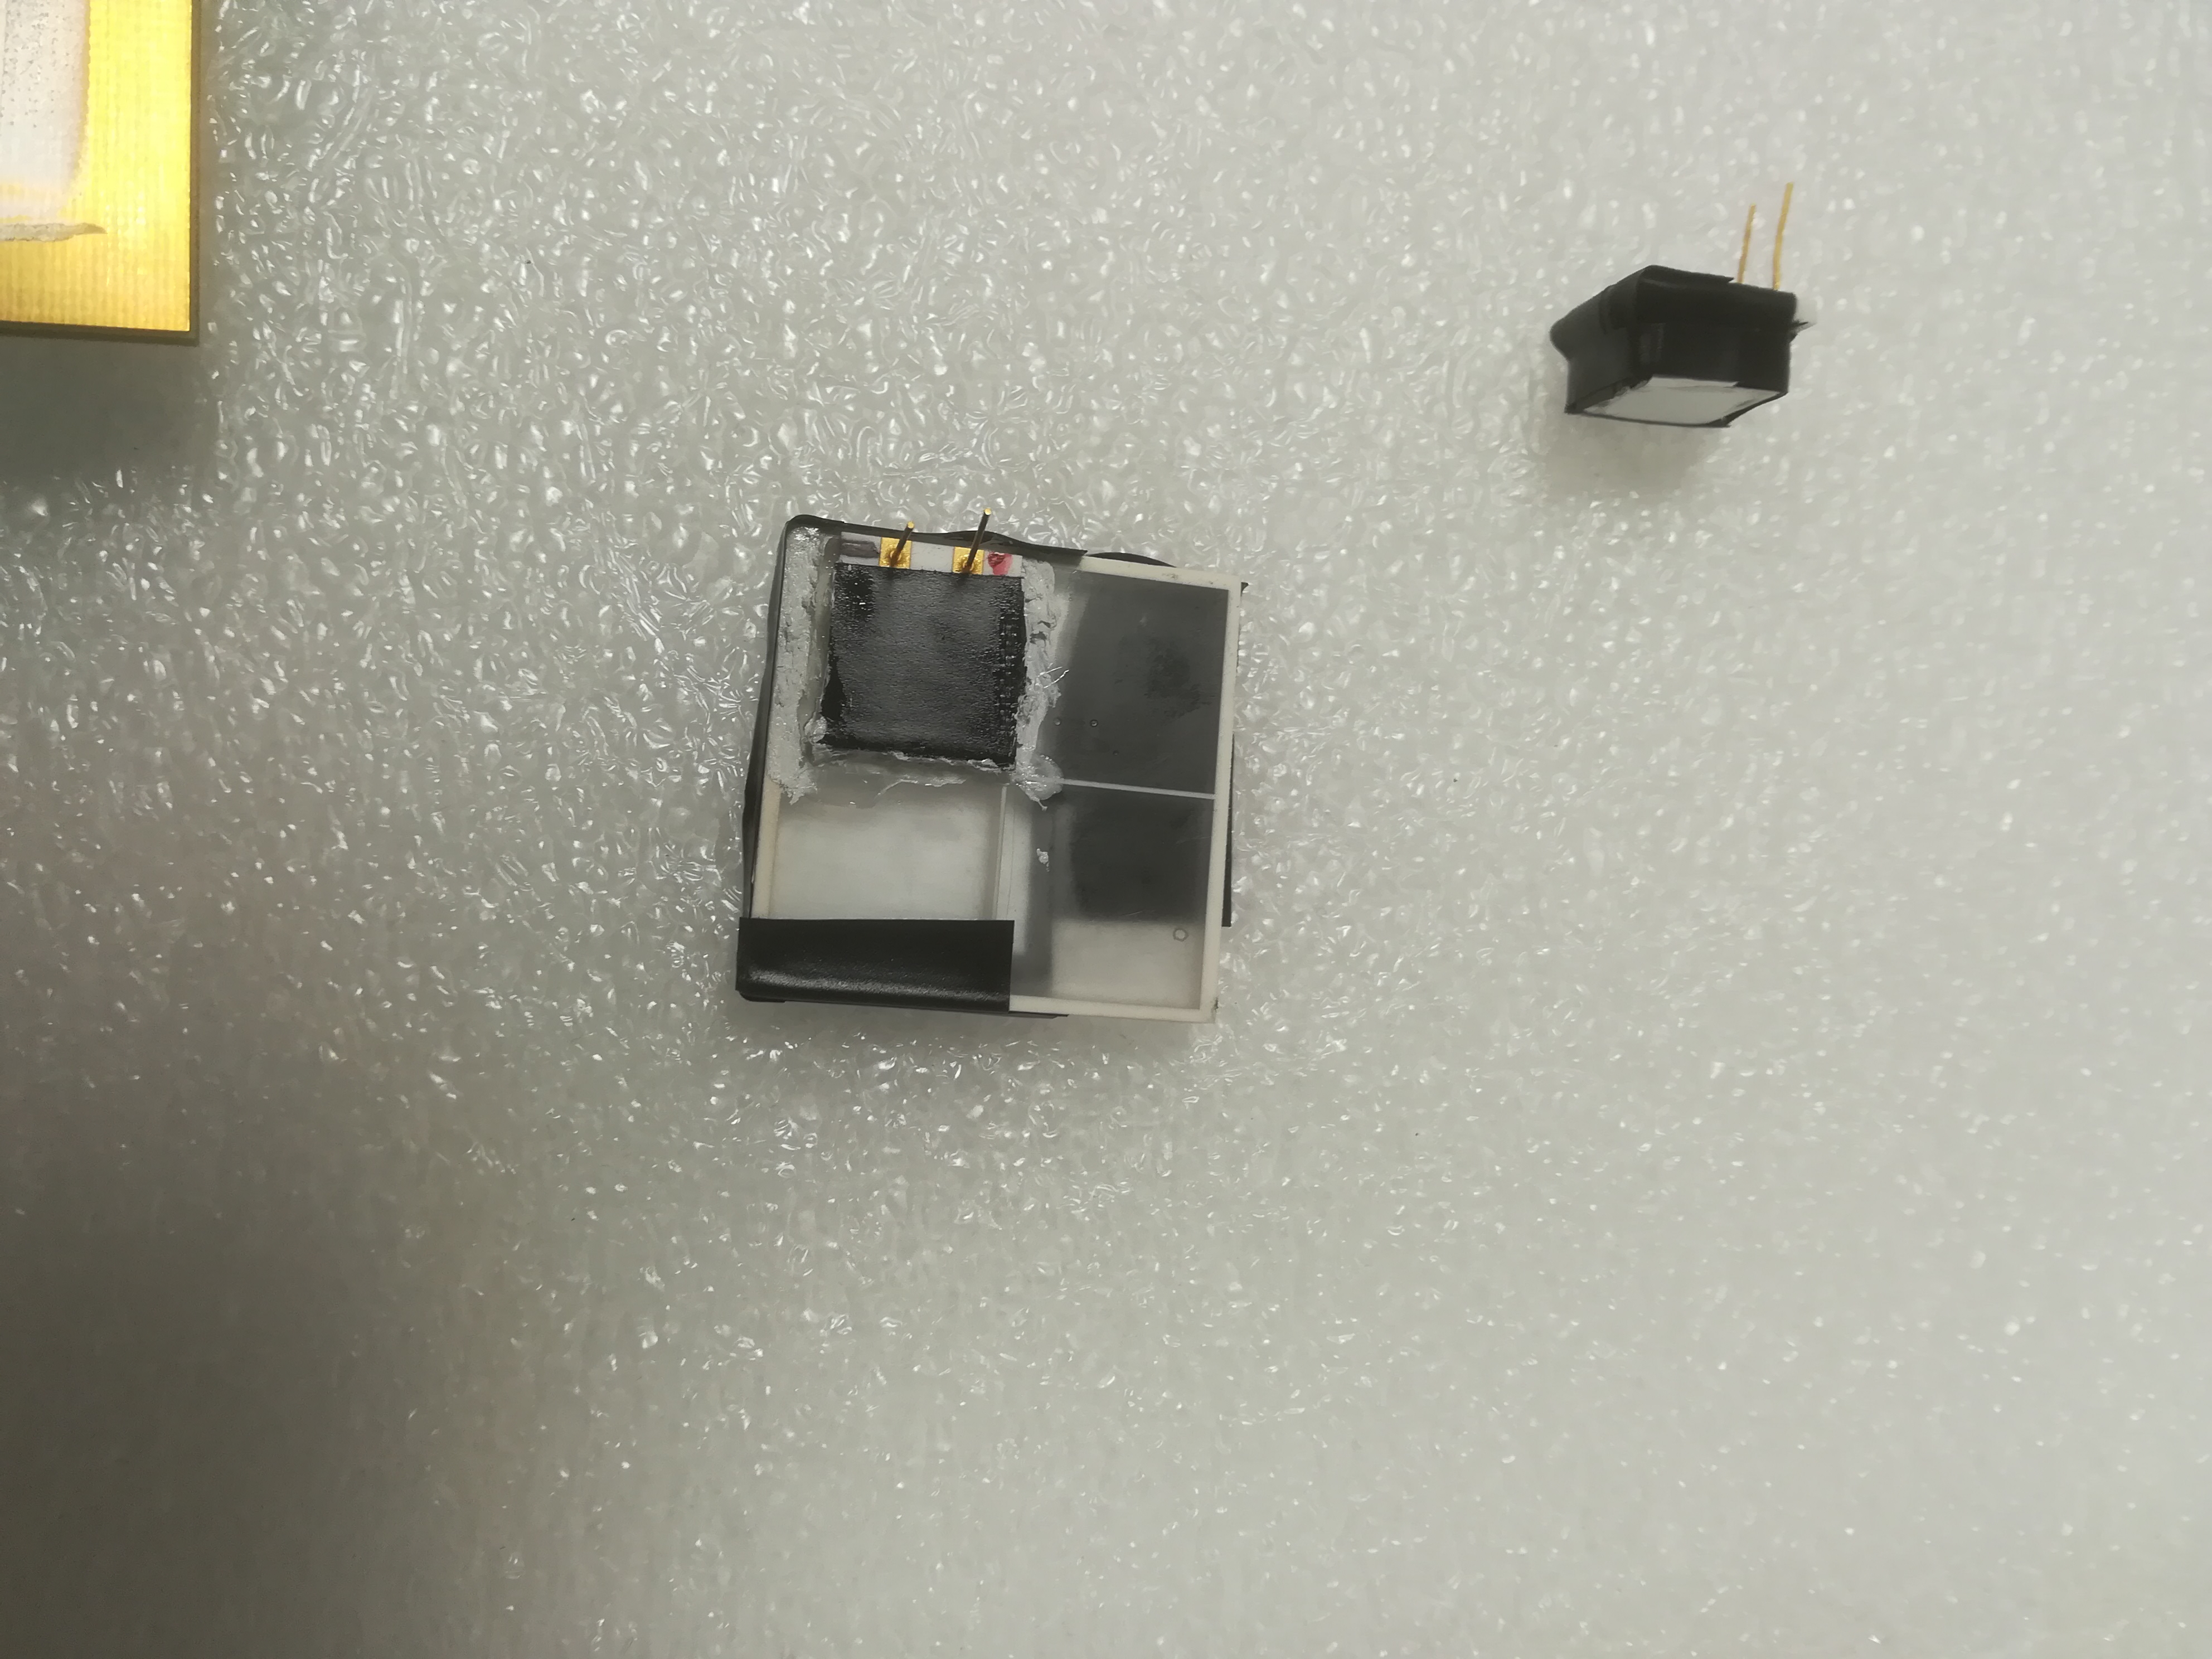
\includegraphics[width=\textwidth, keepaspectratio]{Grafici_Tesi2/Confronto/csi.png}
	\caption{Spettro in $E_{CsI}$: in blu sono rappresentati i dati sperimentali, in rosso quelli simulati. Gli istogrammi sono normalizzati in area.} \label{fig:spettro_csi_confronto}
\end{figure}

L'accordo tra dati sperimentali e simulati è avvalorato dalla complessità della situazione considerata: in primo luogo, la reazione~\ce{^{12}C}(\ce{^{20}Ne},\ce{^{16}O})\ce{^{16}O} avviene in cinematica inversa, così che l'energia cinetica dell'eiettile risulta estremamente sensibile alla variazione dell'angolo di emissione. 
Inoltre, la presenza del substrato epitassiale davanti al volume sensibile del rivelatore al SiC genera fenomeni non-lineari nell'energia.
Infine, la bassa statistica registrata durante il test ha reso importanti le fluttuazioni 

